\section{Estratégias para recepção de novatos.}

Desde sua criação, a Wikipédia viu seu número de usuários ativos crescer ano após ano. Isso foi verdade até XXXX (BUSCAR REFERÊNCIA), quando a tendência de crescimento desacelera, e então a comunidade passa a encolher. 

*** TRAZER DADOS E GRÁFICOS SOBRE NÚMERO DE USUÁRIOS ATIVOS. PODEM SER DO STATS MESMO.

A análise bruta dos dados de engajamento na atividade de escrita nas Wikipédias parece apontar que o crescimento orgânico da comunidade tinha um teto, e a mesma entende que precisa continuar crescendo para cumprir seu objetivo de ``disponibilizar todo conhecimento do mundo'' e para ter mão de obra para garantir os trabalhos administrativos. (BUSCAR REFERÊNCIA)

Além das preocupações mais rasas dos problemas ocasionas pela diminuição na oferta de mão de obra, existe na diminuição da comunidade um problema conceitual que se defront com a missão da Wikipédia: se é entendido que todo conhecimento tem um viés de acordo com quem o produz, a enciclopédia só poderá alcançar seu objetivo de reunir todo o conhecimento humano se todas as pessoas do mundo estiverem a editando. Somente assim ela poderia ter toda a diversidade humana representada. É óbvio que este enunciado é uma hipérbole, mas ele exerce a função de um norte utópico a ser buscado no fazer diário dos wikipedistas, e os mobiliza para pensar em formas de nortear sua ação rumo a esse objetivo.

Seguindo esta bússola, ***Mencionar tentativas de melhorar recepção… Ver https://trello.com/c/6ufGcyAz/339-textos-mencionados-sobre-dificuldade-dos-novatos-para-intro-do-cap%C3%ADtulo

*** Falar da dificuldade de entrar em uma comunidade prática já densa usando citações abaixo.

"a ampla aceitação de artefatos e arranjos organizacionais é condição sine qua non para participar de uma comunidade de prática (Lave and Wenger 1991, Star 1996). Estranhos e pessoas de fora de um grupo têm a infraestrutura como um alvo de aprendizado. Novos participantes adquirem familiaridade com estes objetos à medida que se tornam membros do grupo. (STAR; RUHLEDER, 1996, apud BOWKER; STAR, 2007, p.35)" (FEITOSA, 2010. p. 17) # talvez aproveitar originais desta citação

*** Buscar algo do Primo sobre frustração dos entrevistados dada a dificuldade em colaborar no WP. Citar que essa dificuldade foi observada nas falas de lá, e que iremos atrás de como a Wikipedia faz para tentar minimizar essa situação.

Assim, chegamos ao momento ``quando os de dentro saem''. Em um movimento análogo ao feito por cientistas, que devem sair fisicamente de seus laboratórios para fazer/reforçar enredamentos que irão manter/expandir a sua atuação, os wikipedistas então passam a organizar as chamadas atividades de \textit{outreach}\footnote{Em uma tradução livre ao português poderíamos chamar essas atividades de extensionistas, mas a comunidade lusófona da Wikipédia utiliza em seu cotiano o termo \textit{outreach} em inglês mesmo, portanto seguiremos o utilizando desta forma na pesquisa.}. 

Nestas atividades, editores experientes buscam (BUSCAR REFERÊNCIA OBJETIVOS OUTREACH WIKIMEDIA)

Dentre diversas atividades de extensão realizadas pelo Movimento Wikimedia, destacamos aqui dois grupos de atividades que aparecem concentrar a maior parte de seus esforços: Os projetos GLAM e o Programa de Educação.


\subsubsection{GLAM}

*** Catar alguns autores de outreach para falar sobre glam por alto.

*** Trazer números. Falar sobre como muitas vezes as atividades GLAM apoiam outros projetos Wikimedia, como Commons, Wikisource e Wikidata.

***  Citar o projeto 1lib1ref.
***  Falar que uma das contribuições da pesquisa foi melhoria do código do citation hunt, e sua disponibilização para pt. Trazer números do citation hunt.

*** Citar números dos WL* e mencionar que as ferramentas para monitoramento e avaliação foram criadas pela comunidade brasile

\subsubsection{Programa de Educação}

*** sobre pré-programa de educação citar interesse da comunidade de engajar acadêmicos e pesquisa (TARABORELLI 2011)

*** Falar sobre a história do programa. Quando foi criado, qual sua capilaridade. 

O programa estimula professores a proporem para seus estudantes a edição verbetes da Wikipédia como uma atividade da disciplina. Para apoiar essas atividades, a Fundação Wikimedia cria materiais de apoio e estimula voluntários a apoiarem as iniciativas como embaixadores.
    
***  Quantos cursos em quantos países, bytes adicionados….

*** Sobre o programa de educação, usar (MARQUES, 2012), (CARVER et al., 2012), (ARCHUBY, 2018), (SOLER-ADILLON, 2018)

Observando experiências e relatos de diversas instâncias de turmas universitárias dentro do Programa de Educação, podemos observar de forma explícita a dificuldade de professores e estudantes para criar conteúdos na Wikipédia e suas tentativas de negociação com a comunidade para a criação de estratégias que possibilitassem a permanência dos conteúdos criados pelos estudantes no projeto.(MARQUES, 2012).

Sabemos que conteúdos criados em salas de aula costumam ter dificuldades para permanecer na Wikipédia. São comuns os relatos de professores e alunos desmotivados por verem suas contribuições desaparecerem do ar pouco depois de serem salvas. Os casos mais repetidamente vistos como bem sucedidos adotam estratégias para tentar mitigar essa situação, como por exemplo estimular os alunos a editar primeiro em uma página de testes, onde o conteúdo será revisado pelo professor e por outros voluntários, para só então ser adicionado à página do verbete desejado.

Assim por exemplo foi feito por Juliana Bastos Marques, professora da UNIRIO, responsável pelo primeiro caso de instanciamento do Programa de Educação da Wikimedia Foundation no Brasil. Como relatado por ela na Revista História Hoje (2012, p. 339), ``uma maneira bastante segura de evitar conflitos com wikipedistas durante a realização da disciplina é fazer que os alunos escrevam seus artigos apenas em suas páginas de teste, e que após a avaliação eles sejam corrigidos pelo/a professor e embaixadores, para que então possam ser ‘colocados no ar’. Este modelo não é consenso entre os professores que adotaram o projeto até agora, mas se provou fácil e seguro". Corroborando com nossa experiência, a autora afirma no mesmo texto que “observou-se que outros cursos já ministrados no Brasil dentro do mesmo projeto não conseguiram alcançar resultados satisfatórios no mesmo grau'' (MARQUES, 2012. p. 338).

Sabendo das dificuldades encontradas por essa estratégia (BUSCAR REFERÊNCIAS) de articular com docentes no Brasil a escrita de verbetes Wikipédicos, possivelmente associada a dificuldade de ter a figura do embaixador de campus dadas as diferenças entre a vida de um universitário brasileiro e um norte-americano (BUSCAR REFERÊNCIA), passamos a olhar então para atividades que, mesmo sendo realizadas muitas vezes dentro dos \textit{campi} universitários, não fazem parte do arcabouço do Programa de Educação.

\subsection{As Editatonas}

*** Para falar de editatonas citar (CAMPANY e KAHILI-HEEDE, 2018), (FARZAN et al. , 2016), (LITTLEJOHN, Allison et al., 2019), (MARQUES e LOUVEM, 2013)

Uma das principais formas que o Movimento Wikimedia tem para engajar e trazer novos/as usuários/as à comunidade são as editatonas. Realizadas por todo o mundo, são eventos onde pessoas se reúnem para editar sobre um mesmo tema de interesse. Como definida pela própria enciclopédia, no verbete ``Maratona de edição'' na Wikipédia em português, uma editatona é um evento ``\textit{durante o qual editores se reúnem para editar e melhorar um tema ou tipo específico de conteúdo, geralmente incluindo um treinamento em edição básica para novos editores. A palavra é uma combinação das palavras ``editar'' (\textit{edit}) e ``maratona'' (\textit{marathon})}'' \citewiki{ptwiki_maratona}.

*** Editatonas: falar da ambiguidade do termo em inglês e da perda na tradução.

*** Falar aqui que é uma forma de atividade que perpassa atividades de educação, de glam, wiki projetos e outras iniciativas avulsas, inclusive tendo Learning Patterns "próprios", compartilhados por extensionistas de diversas frentes do movimento.

\begin{figure}[H]
    \centering
    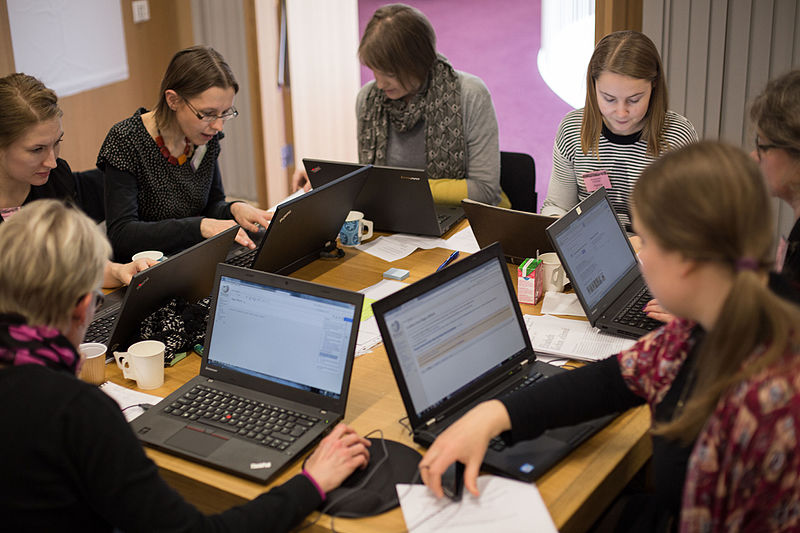
\includegraphics[width=1\textwidth]{Images/editatona_antiga.jpg}
    \caption{Exemplo de uma editatona presencial sendo realizada.}
    \label{fig:editatona_antiga}
\end{figure}

Há variações em seu formato, mas normalmente a atividade começa com um (ou mais) editor/a(es/as) experiente(s) apresentando o funcionamento da enciclopédia e introduzindo suas políticas editoriais. Em sequência, os/as demais participantes criam uma conta de usuário/a e começam a escrever, individualmente ou em grupo, verbetes de seu interesse. Nesta fase, o/a(s) usuário/a(s) experiente(s) atua(m) como tutor/a(es/as), tirando dúvidas dos/as novatos/as que apareçam durante o processo de edição.

Existem também algumas editatonas que funcionam como ``forças-tarefas'' de usuários experientes melhorando verbetes sobre um determinado assunto focal, como por exemplo ``patrimônio natural brasileiro''\footnote{https://pt.wikipedia.org/wiki/Wikipédia:Edit-a-thon/Atividades\_em\_português/Wiki\_Loves\_Earth\_Brasil\_2015 , acessada em 19 de março de 2020.} ou ``eleições no Brasil''\footnote{https://meta.wikimedia.org/wiki/Programa\_Catalisador\_do\_Brasil/2013-2014/Micro-subsídios/Solicitação/Wikitona\_Eleições\_2014 , acessada em 19 de março de 2020.}. Estas atividades dispensam a explanação inicial, e, os/as presentes, editores/as já experientes, partem rapidamente para a divisão de tarefas e escrita de conteúdos. Habitualmente, essas forças tarefas são realizadas online, e a maioria das editatonas presenciais é direcionada em apresentar o mundo wiki a novos/as editores/as a partir de assuntos que sejam de seu interesse.

No início de 2020, a página para divulgação de editatonas da Wikipédia em português já contava com 120 eventos cadastrados desde 2013, sendo 115 deles (98,5\%) realizados no Brasil\citewiki{ptwiki_edit_a_thon_atividades_portugues}. Já na página para editatonas da Wikipédia em inglês, estavam mapeados 121 eventos, com o primeiro datando de janeiro de 2011 e o último de maio de 2018\citewiki{enwiki_how_run_edit_a_thon}, indicando que provavelmente essa comunidade passou a registrar seus eventos realizados no último ano e meio em outro lugar. Já a Wikipédia em espanhol apresentava 92 eventos\citewiki{eswiki_editaton}, mas aparentemente México, Argentina e Espanha, pólos movimentados de atividade wiki, estão com seus números desatualizados. Terminando nosso passeio pelas páginas sobre editatonas das maiores Wikipédias do mundo, encontramos 60 atividades mapeadas na versão francófona (com destaque para um evento realizado recentemente em Guiné, o primeiro fora do eixo França-Canadá)\citewiki{frwiki_journées_contributives} e 83 na enciclopédia em alemão\citewiki{dewiki_edit_a_thon}.

Se por um lado nossa breve busca não conseguiu números precisos sobre a quantidade de editatonas realizadas pelo mundo, entendemos que os valores encontrados já são suficientes para indicar a relevância deste tipo de evento para o Movimento Wikimedia. Eles também indicam que, além da organização destes eventos ser uma estratégia muito utilizada por todo o mundo, ela é especialmente popular no Brasil. Com essa constatação, elegemos então as editatonas como o método a ser acompanhado por nossa pesquisa para observar \textit{in loco} a chega de novos usuários à enciclopédia.
